
In the previous chapter it was shown that the model is accurate, fast, and numerically sound. Then it was shown that the model can reproduce experimental influenza virus and SARS-CoV-2 experiments from real data. In this chapter, the findings, model extensions, and future work of this thesis will be discussed. I will discuss how the faster speed of the simulations allows for the model to be compared with common practices in the field of computation virology, how the current limitation of a lack of all the cell processes can be addressed, and how the model will be applied in the future.

\section{Findings} \label{findings}

\subsection{Advances in ABM simulation}

In this paper, the construction of a hybrid ABM/PDM model to investigate spatially extended viral infections is described. While the formulation of the model is similar to other ABM/PDM models of viral spread \citep{beauchemin_simple_2005, bauer_agent-based_2009}, the model was implemented to run on GPUs, vastly improving the simulation speed of these models. This allows for efficient replication of \emph{in vitro} infections with a realistic number of cells. This will help lead to a better understanding of virus-cell dynamics \emph{in vitro} \citep{blahut21}, but could also help realize the goal of simulating infections \emph{in vivo} \citep{laubenbacher21}. The faster simulations also allowed for the use of standard ordinary differential equation (ODE) model-fitting techniques to fit this model to experimental data, making it possible to quickly parameterize these models to reproduce dynamics of different viruses. Previously, researchers have had to develop other techniques to help speed up fitting of ABMs to experimental data, including reducing the sampled parameter space \citep{li17}, and mapping of ABM outputs to simpler functions \citep{tong_development_2015, read16}. These techniques coupled with simulation of ABMs on GPUs could potentially allow for real-time parameter estimation of models for use in patient care. This is particularly useful for a novel pandemic virus that can be simulated such that trial runs of test drugs can be performed and viral infection severity for a patient can potentially be predicted.

This paper shows that the use of GPUs to accelerate computation of agent-based and partial-differential equation hybrid models allows for simulation results within hours, but with the necessary level of detail to capture individual cell effects, and allows for parameterizing the model quickly. The model in this work accurately replicates the diffusion of a virus, the stages of infection of individual cells, and can be fit to data within hours. While still lacking some of the biology needed for replication of \emph{in vivo} infections, the speed of computation leaves room for incorporation of additional features. Thus, this model implementation forms the foundation of a modeling and simulation tool that can accurately predict in-host viral dynamics and be quickly deployed to help combat the next pandemic. 

\subsection{ABM viral dynamics}

From the data fitting results shown in section \ref{result_fit}, some of our parameter estimates differ from those reported in Pinilla et al.\ \citep{pinilla12} even though the same data was used. Our best fit $\tau_I$ is smaller than the $\tau_I = \SI{49}{\hour}$ reported by Pinilla et al., while our best fit $\tau_E$ is larger than the $\tau_E = \SI{6.6}{\hour}$ found by Pinilla et al., and the best fit $c$ is larger than $c = \SI{0.13}{\per\hour}$. Some of this discrepancy might be due to the inclusion of spatial effects in the ABM, but Pinilla et al.\ also used more data --- they used both a single cycle and multiple cycle experiment as well as viral RNA measurements --- to constrain the parameter estimates. All in all, the ABM/PDM model can replicate the viral titer measurements of a typical infection (both influenza virus and SARS-CoV-2) via fitting where the fitting process uses standard packaged fitting algorithms and the computational time for fitting is less than 24 hours from initial guess to best fit.

In figure \ref{fig_FitRuns}, one might notice that the simulated experiments of the Pinilla et al.\ data vary from each other more than each simulation of the Wang et al.\ data. This is due to the fact that the standard deviation of the Erlang distribution that determines the eclipse phase lengths is dependent on $\tau_E$. The mean of the phase time for the eclipse phase is $\tau_E$ and the standard deviation is $\tau_E/\sqrt{\eta_E}$. Therefore, the standard deviation becomes smaller as $\tau_E$ becomes smaller. This point is illustrated in figure \ref{fig_tauEdis}, where, on the left, the Erlang distributions of the eclipse phase lengths and, on the right, the Erlang distributions of the infectious phase lengths are plotter for each of the three infections. This implies that, for cell free transmission of a virus with a small mean eclipse phase length, the variation in end times of infections for the same virus comes from the differences in infectious phase lengths.

\begin{figure}
\centering
    \resizebox{\textwidth}{!}{%
    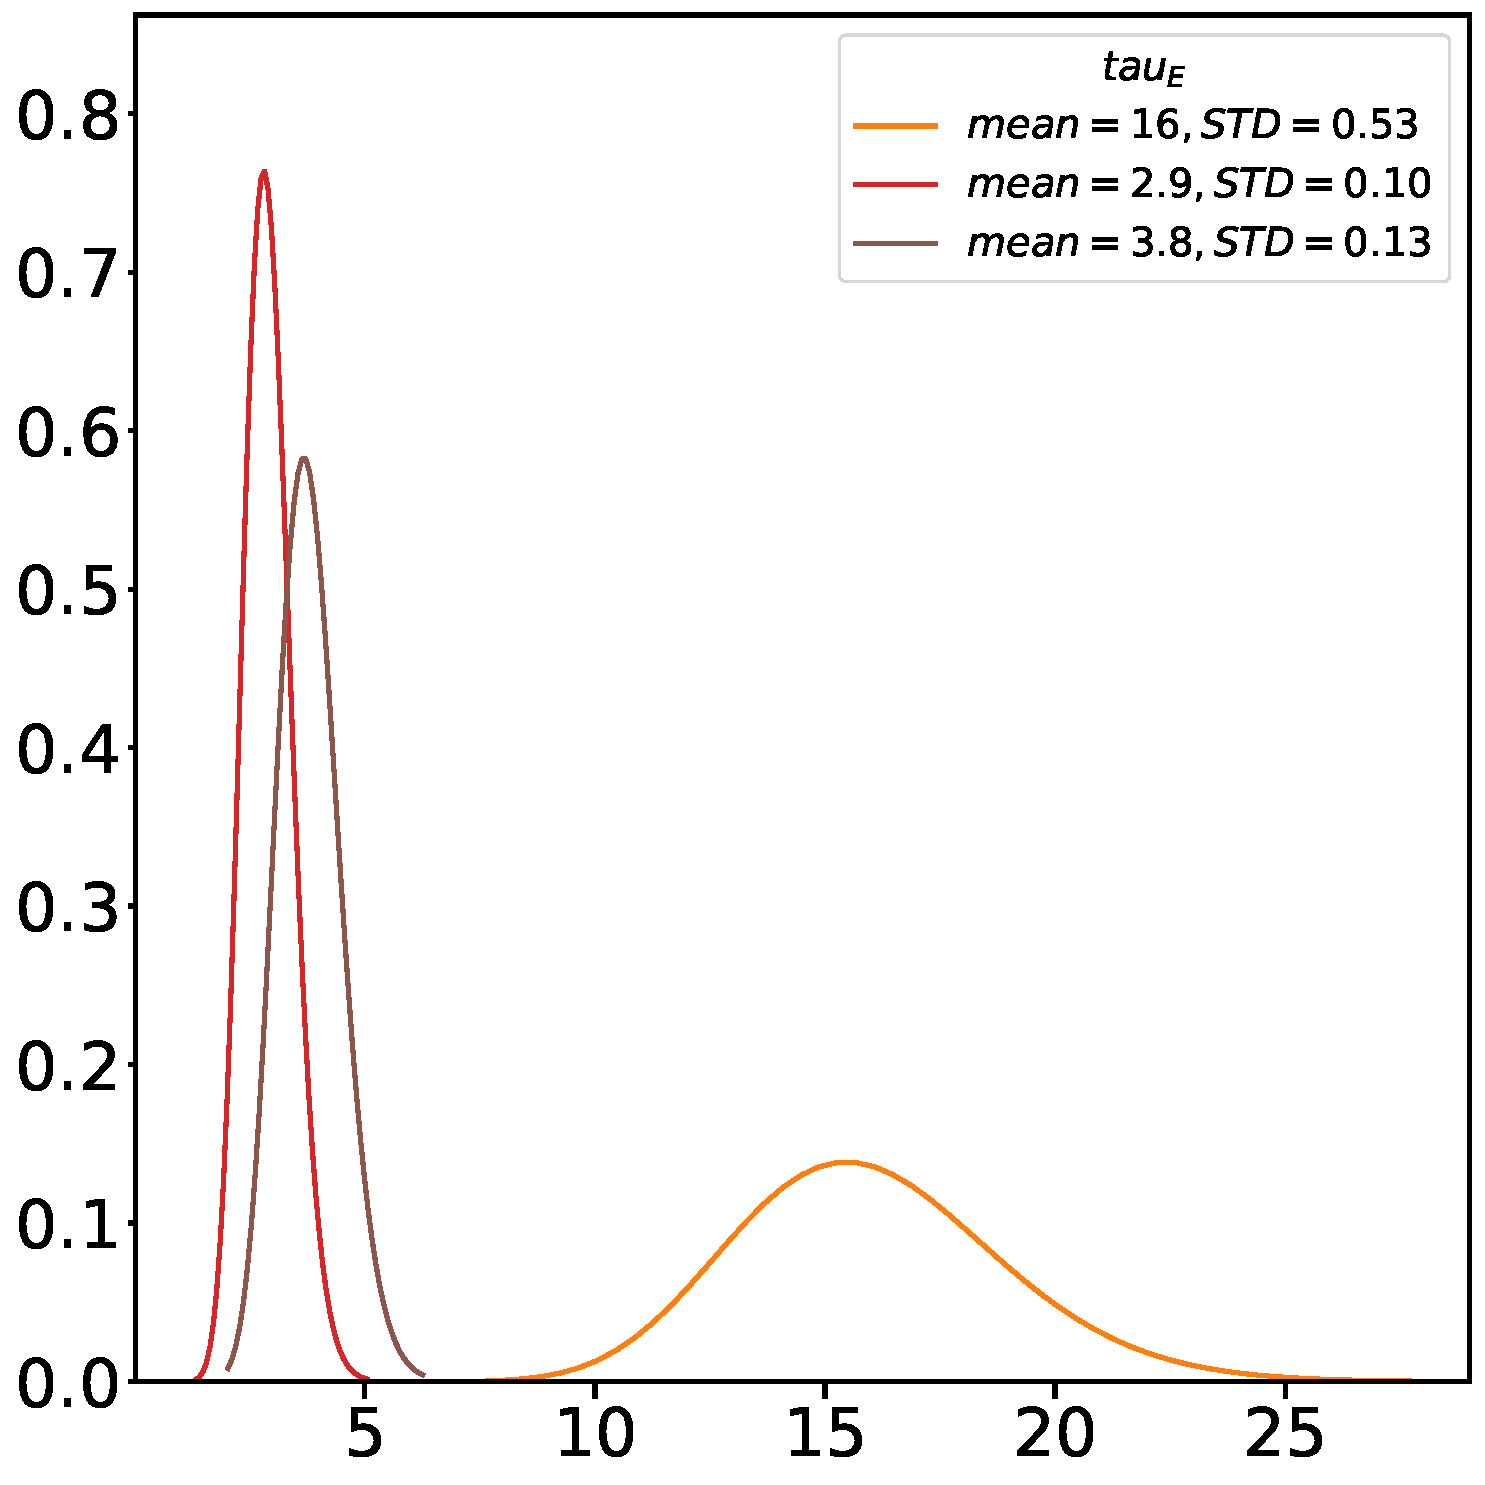
\includegraphics[width=0.48\linewidth]{Figures/tauE.pdf}
    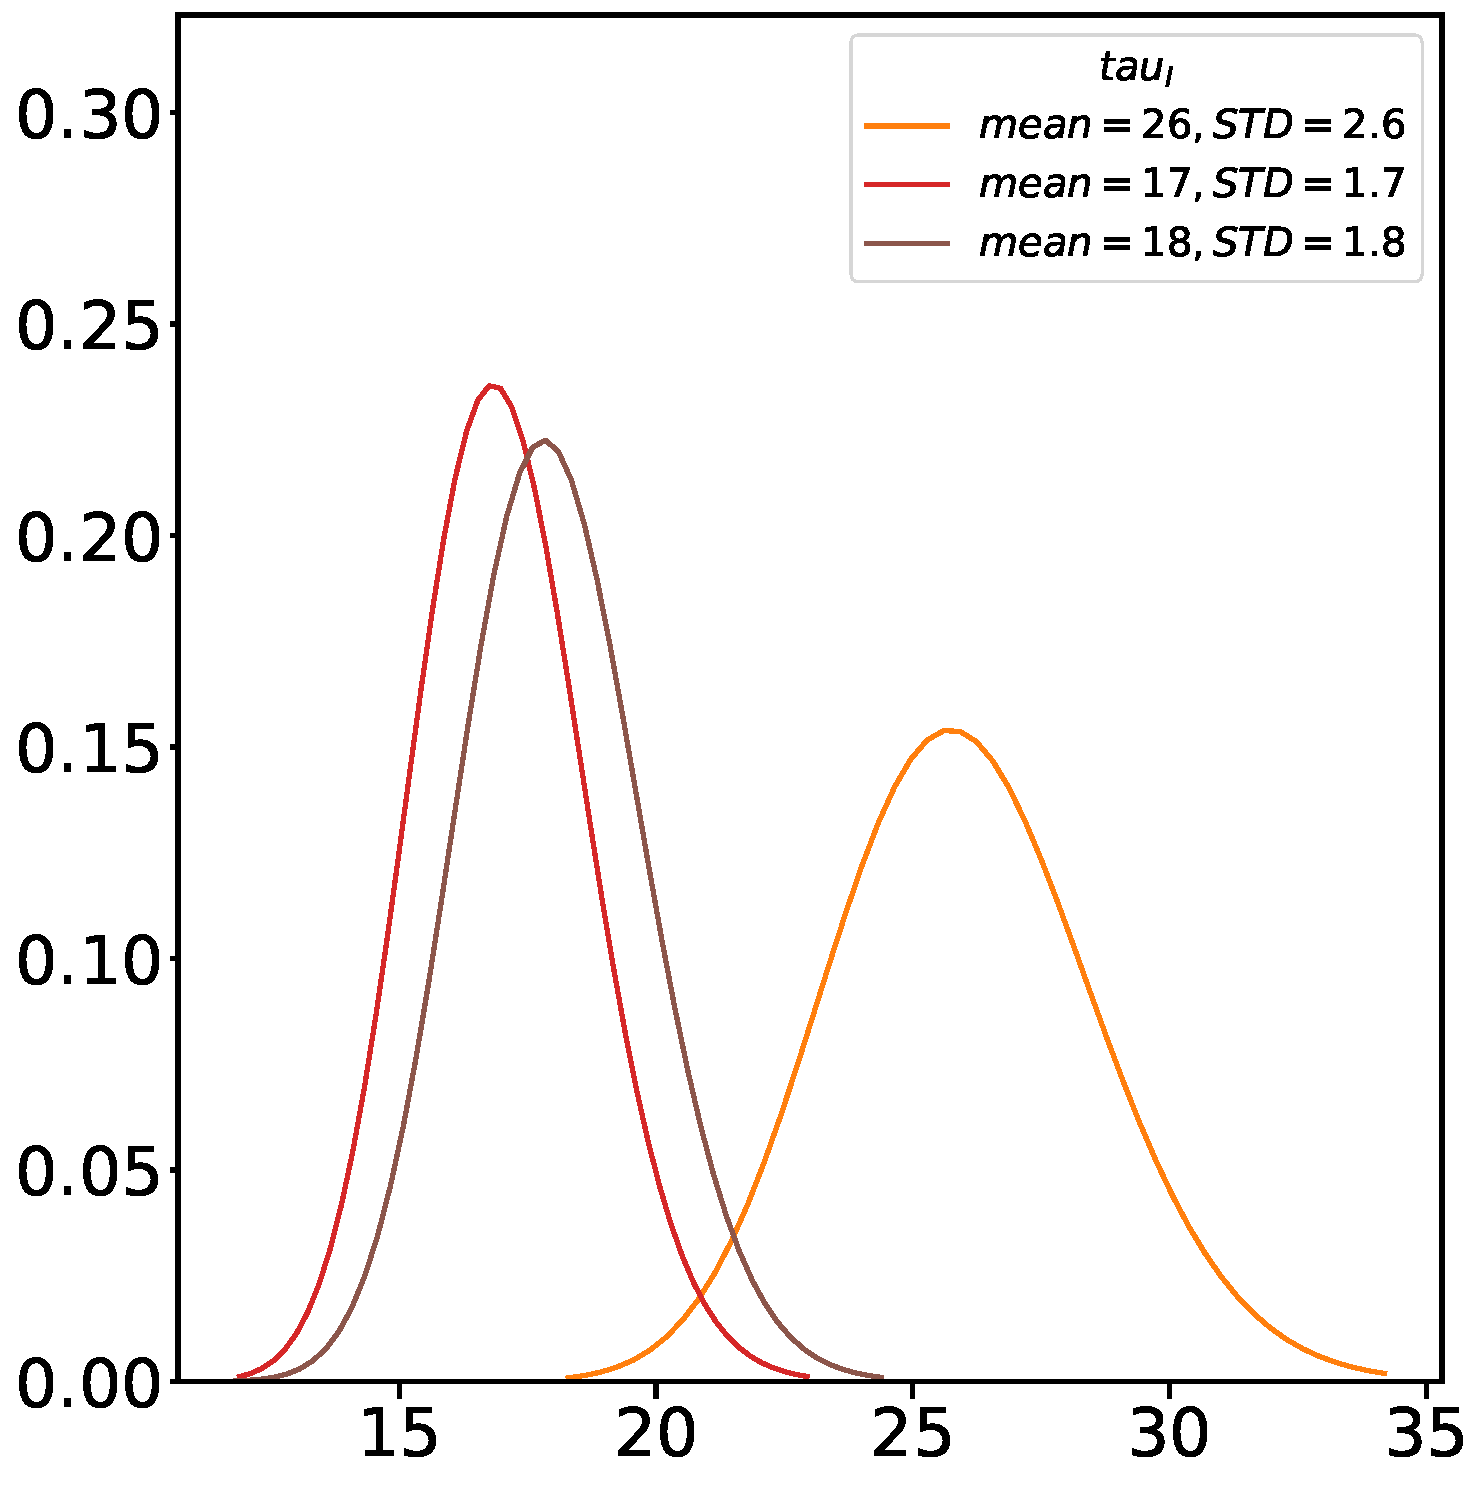
\includegraphics[width=0.48\linewidth]{Figures/tauI.pdf}}
\caption{On the left is the Erlang distributions of the eclipse phase lengths and on the right is the Erlang distributions of the infectious phase lengths. For the eclipse phase and the infectious phase: MEAN $= \tau$ and STD $= \tau/\sqrt{\eta}$. \label{fig_tauEdis}}
\end{figure}

%From table \ref{tab_datafit_params}, $\tau_E$ and $\tau_I$ for the Pinilla et al.\ data are \SI{16}{\hour} and \SI{26}{\hour}, the Wang et al.\ Vero76 data are \SI{2.9}{\hour} and \SI{17}{\hour}, and the Wang et al.\ Vero data \SI{3.8}{\hour} and \SI{18}{\hour}. 


\section{Model extensions}

Although the model currently only incorporates cell-free transmission, since the ABM models interactions of each cell in a culture dish, the spatial aspects of different viral transmission routes can be explored in detail. There has been recent interest in viruses that transmit via cell to cell transmission, with ODE \citep{allen15,komarova13,iwami15}, stochastic \citep{graw15}, and ABM \citep{kumberger18,blahut21} models developed to study how cell to cell transmission alters infection dynamics. There are also viruses that cause cells that form syncytia, which are cells that have fused into a single multi-nucleated cell. Not much is known about how syncytia alter infection dynamics, with a recent ODE model attempting to assess the effect of syncytia on viral time course \citep{jessie21}, but spatial effects really need to be included for a proper assessment of the role of syncytia. Finally, advection can be added to the diffusion of the virus particles to more closely mimic the respiratory tract. Recent PDE \citep{quirouette20} and ODE \citep{gonzalez19} models both indicate that the addition of advection can limit the spread of respiratory viruses towards the lower respiratory tract, but the stochasticity included in an ABM might affect this result. 

While the model is able to replicate a typical viral time course during an infection, it is missing many components that play important roles in the infection. For example, the immune response of the host has not been added to the model. The immune response is a large, if not the main, contributing factor to symptoms experienced during a viral infection \citep{manchanda14,zheng18}, but also limits spread of infection itself \citep{dobrovolny13}. ABMs are already used to model various aspects of the immune response \citep{whitman20,kerepesi19,levin16}, so the immune response can be incorporated into the existing ABM/PDM framework. Cell tropism, the preference of virus for one cell type over another, is another feature of viral infections that can be incorporated into the ABM. ODE modeling indicates that cell tropism can lead to longer lasting infections \citep{dobrovolny10}, but will also likely affect the spatial dynamics of infection. Finally, variation in production of virus by individual cells \citep{timm12} can be incorporated to determine how this type of cell heterogeneity affects spatiotemporal infection dynamics.

%%%%%%%%%%%%%%%%%%%%%%%%%%%%%%%%%%%%%%%%%%%%%%%%%%%%%%%%%%%%%%%%%%%%%%%%%%%%%%%%%%%%%

\section{Future Work}

A goal of this research is to not only be able to predict viral infection, but it is to find ways to uncover potential causes of disease severity. The novel coronavirus, SARS-CoV-2, originated in Wuhan, China in late 2019 and rapidly spread around the world \citep{chen20,wu20}. This virus causes the Covid-19 disease, which can lead to severe illness needing long hospitalization \citep{sun20,goyal20,jiang20}, but at the same time a significant fraction of those who contract the virus experience an asymptomatic Covid-19 disease \citep{he20}. It is still not entirely clear who is at risk for developing severe disease, although correlations of disease severity with levels of vitamin D \citep{ilie20}, levels of various immune components \citep{liu20imm,liu20imm2,zhang20imm,yang20imm}, and age \citep{borghesi20,zhang20imm} have been noted. There has also been investigation of the possibility of disease severity being linked to initial viral inoculum \citep{little20, guallar20, ghandi20}.

The difference in viral inoculum between patients could be caused by varying amounts of virus in airbone droplets. The major route of transmission for SARS-CoV-2 is by airborne droplets \citep{morawska20}. One study indicates that sneezing and coughing creates a turbulent gas cloud that can cause viral-laden droplets to spread up to 27 feet (\numrange[range-phrase = --]{7}{8}\si{\meter}) \citep{bourouiba20}, and allows the virus to get into the ventilation system of a building. A review of literature on droplet and airborne viral spread concludes that 8 of 10 studies showed that droplets spread further than the 6 foot \citep{bahl20} social distancing recommendation. While personal protective equipment is helpful in reducing the ability of virus to enter the respiratory tract, it is not perfect \citep{mittal20}. All of these factors lead to exposures to vastly different quantities of virus when people are going about their daily activities. Thus it is important to understand whether different initial inocula lead to different viral dynamics in patients. 

There is some evidence from other respiratory viruses that the size of the initial inoculum could play a role in the severity of the illness. An influenza epidemiological modeling study suggests that a higher initial dose can lead to a higher mortality rate \citep{paulo10}. This is corroborated by an influenza in-host modeling study that also finds a correlation between the initial viral dose and survival rate \citep{price15}. Other modeling studies have found dependence of other measures of infection severity on initial dose for influenza \citep{moore20}, respiratory syncytial virus \citep{wethington19}, adenovirus \citep{li14}, and porcine reproductive and respiratory virus \citep{go19}. There are also experimental studies that find a link between dose and infection severity. Experiments using influenza have found inoculum dose dependence of total number of infected cells and area under the curve \citep{manicassamy10}, peak viral titer \citep{ginsberg52,iida63,ottolini05}, viral growth rate \citep{ginsberg52}, and time of viral peak \citep{iida63,ginsberg52}. Experiments with other viruses, such as adenovirus \citep{prince93}, and parainfluenza \citep{ottolini96}, have also shown correlations between initial inoculum and various measures of disease severity. If SARS-CoV-2 shows a similar pattern, initial inoculum should be considered as a possible contributor to infection severity and adverse outcomes. With this model different scenarios can be tested to help narrow down and rule out causes a different viral infection severities. 

\section{Conclusion}

In this thesis, I've presented the testing, validation, and application of a GPU accelerated, hybrid, agent-based and partial differential equation model. I demonstrated that the model incorporates the spatial spread of viruses and produces accurate simulations in a few seconds or minutes, by utilizing parallel processing on GPUs. From the speed increase, standard model-fitting techniques, such as ``Minimizing the SSR'', can be used to fit the model to experimental data. Now viruses can be studied in a more accurate way and parameterized in hours. By creating this model, the foundation of a modeling and simulation tool has been developed to study viruses. This work will be deployed to study different aspects of a virus, how different viruses affect infection, and what may lead to different severities of infections. Now that I've created a new in-host viral model, when the next flu season, epidemic, or pandemic comes; there will be one more tool that can help to gain insight and hopefully help end or slow the spread of the virus.












